\section{本章小结}

多重积分在数学上是一个$n$元函数在$n$维空间的积分。
\begin{figure}[h]
\centering
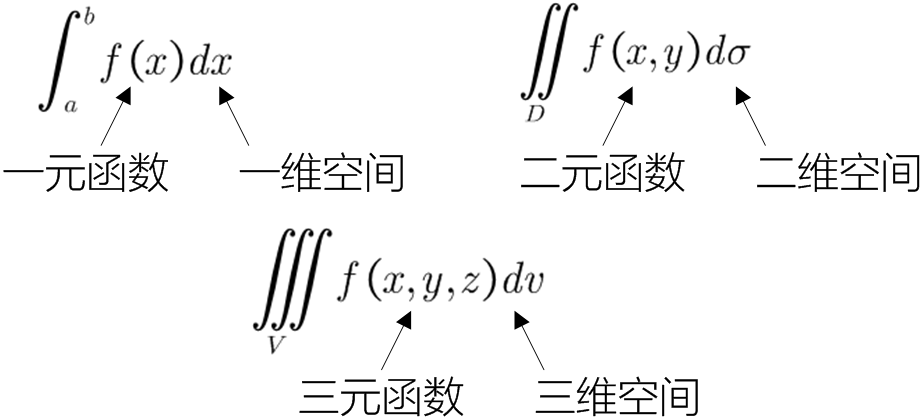
\includegraphics[height=3.5cm]{8.4.png}
\end{figure}

多重积分的物理意义非常简单明了,即已知$n$维体的体密度,求解该$n$维体的总重量。
如下表示线重量、面重量、体重量:
\begin{align*}
&W=\int_a^b{\rho \left( x \right) dx} \\
&W=\iint\limits_D{\rho \left( \boldsymbol{p} \right) d\sigma} \\
&W=\iiint\limits_V{\rho \left( \boldsymbol{p} \right) dv}
\end{align*}

多重积分的计算,总体步骤也非常明了:
\begin{enumerate}
    \item 固定$n-1$维,剩下一维变量进行积分,相当于求解一个一元函数积分,只是积分上下限是一个包含其余$n-1$维变量的表达式;
    \item 继续反复上面的步骤,直到剩下一维;
    \item 求解该一元积分。
\end{enumerate}
被积函数(即权重函数、或称密度函数)是给定的。
难点在于确定各个维度的积分上下限,即对于给定的积分区域求解各个维度的相互关系。




